\documentclass[14pt,aspectratio=169,hyperref={pdftex,unicode},xcolor=dvipsnames]{beamer}
\usepackage[english,russian]{babel}
\usepackage[utf8x]{inputenc}
\usepackage[T2A]{fontenc}
\usepackage{cmap}
\usepackage{paratype}
\usepackage{minted} % для примеров кода (требует параметра -shell-escape)
\usepackage{listings, lstautogobble}

\usepackage{multirow}
\usepackage{tabularx}
\usepackage{multicol}

\usetheme{metropolis}
\usefonttheme[]{professionalfonts}  % запрещаем beamer'у перезаписывать мат. шрифты
\metroset{numbering=fraction}
\metroset{subsectionpage=progressbar}

\setbeamercolor{frametitle}{fg=black}
\setbeamertemplate{frametitle}
{
 \vspace{3mm}\insertframetitle\par
}
\setbeamertemplate{title separator}{}
\setbeamertemplate{footnote separator}{}


\usebackgroundtemplate{
\includegraphics[width=\paperwidth,height=\paperheight]{./common/background_white.jpg}}

\logo{\vspace{-1.2cm}
\includegraphics[width=6mm]{./common/short-v.pdf}\hspace*{1.08\textwidth}}

\colorlet{mygray}{black!30}
\colorlet{mygreen}{green!60!blue}
\colorlet{mymauve}{red!60!blue}

\lstset{
    backgroundcolor=\color{gray!10},  
    basicstyle=\small,
    columns=fullflexible,
    breakatwhitespace=false,      
    breaklines=true,                
    captionpos=b,                    
    commentstyle=\color{mygreen}, 
    extendedchars=true,              
    frame=single,                   
    keepspaces=true,             
    keywordstyle=\color{blue},      
    language=MetaPost,                 
    numbers=none,                
    numbersep=5pt,                   
    numberstyle=\tiny\color{blue}, 
    rulecolor=\color{mygray},        
    showspaces=false,
    showstringspaces=false,
    showtabs=false,                 
    stepnumber=5,                  
    stringstyle=\color{mymauve},    
    tabsize=2,
    autogobble=true,
    title=\lstname
}

\lstnewenvironment{code}
{\minipage{\linewidth}\vspace{25pt}}
{\endminipage}

\hypersetup{urlcolor=blue, colorlinks=true}

\institute
{
  \begin{columns}
    \begin{column}{1.5cm}
    
\includegraphics[height=15mm,keepaspectratio]{./common/math-cs.pdf}
    \end{column}
    \begin{column}{4cm}
          Факультет математики и компьютерных наук СПбГУ
    \end{column}
  \end{columns}
}


\begin{document}

\begin{frame}[plain]
  \begin{center}
    \textbf{Владимир Рачкин и Павел Балай}

    {\Large\textbf{Построение TLA\textsuperscript{+} модели для смарт-контракта Phoenix Vault}}

    Проект по курсу математической логики, весна 2022

    %{\small Научный руководитель: А.\,А.\,Выбегалло}

    04.06.2022
  \end{center}


  \begin{columns}
    \begin{column}{1cm}
    
\includegraphics[height=15mm,keepaspectratio]{./common/math-cs.pdf}
    \end{column}
    \begin{column}{10cm}
      \small
          Факультет математики и~компьютерных наук СПбГУ\\
          Программа <<Современное программирование>>
    \end{column}
  \end{columns}
\end{frame}



\begin{frame}
\frametitle{Постановка задачи}
\begin{enumerate}
\item Изучить смарт-контракт, описанный в статье\footnote{ \href{https://arxiv.org/abs/2106.01240}{Phoenix: A Formally Verified Regenerating Vault (2021) за авторством Uri Kirstein, Shelly Grossman, Michael Mirkin, James Wilcox, Ittay Eyal, Mooly Sagiv}} 
\item Построить его TLA+ модель и проверить свойства
\item Cмоделировать специальные события: потери ключа и атаки злоумышленника
\end{enumerate}
\end{frame}

\begin{frame}{Что такое Phoenix Vault}
    Это обёртка для Etherium-кошелька
    \begin{itemize}
    \item 2 тира ключей: обычные - для отправки средств, привилегированные - для управления контрактом
    \item Возможность создавать новые ключи и удалять старые
    \item Задержка перед отправкой средств
    \item Возможность отменить отправку средств
    \item Возможность заблокировать отправку средств
    \end{itemize}
\end{frame}

\begin{frame}[fragile]
\frametitle{Модель}
\begin{multicols}{2}
\begin{center}
\small
\begin{tabular}{ | l | c |}
\hline
Action & Key \\
\hline
Deposit & \\
Request  & $T_2$\\
Withdraw & \\
Cancel request  & $T_1$\\
Cancel all requests  & $T_1$\\
Cancel self request & $T_2$ \\
Lock  & $T_1$ \\
Add a $T_1$ key & $T_1$ \\
Add a $T_2$ key & $T_1$ \\
Remove a $T_2$ key & $T_1$ \\
\hline
\end{tabular}
\end{center}

\begin{center}
\small
\begin{tabular}{ l c }
Events: & \\
Tier-1 Key Loss & \\
Tier-2 Key Loss  & \\
Type-1 Attack & \\
Type-2 Attack & \\

\end{tabular}
\end{center}
\end{multicols}
\end{frame}

\begin{frame}[fragile]
\frametitle{Состояния модели}
\small
\begin{itemize}
    \item balance          
    \item block\_number                    
    \item tier\_one\_addresses             
    \item tier\_two\_addresses              
    \item delay              
    \item unlock\_block 
    \item requests     
\end{itemize}

\end{frame}

\begin{frame}[fragile]
\frametitle{Хранение предыдущего действия}
\begin{code}
Lock(address1, new_unlock_block) ==
    /\ previous_command' = (<<"lock", address1>>) 
	...
    /\ unlock_block' = new_unlock_block
    /\ UNCHANGED <<balance, tier_one_addresses, tier_two_addresses, delay, requests, special_vars>>

OnlyTierOneCanLock ==
    [][previous_command'[1] = "lock" => previous_command'[2] \in tier_one_addresses]_previous_command
\end{code}
\end{frame}

\begin{frame}[t]{Достижимость состояния}
\begin{itemize}
\item<1-> $A$
\item<2-> $\neg A$
\item<3-> $\square(\neg A)$
\item<4-> $\neg \square(\neg A)$
\item<5-> $B \Rightarrow \neg \square(\neg A)$
\item<6-> $\square(B \Rightarrow \neg \square(\neg A))$
\end{itemize}
\end{frame}

\begin{frame}[fragile]
\frametitle{Достижимость состояния 2}
\small
\begin{code}
TierOneCanCancelAnyRequestAnyTime ==
[]((requests /= {} /\ block_number < MAX_BLOCK_NUMBER) => 
        LET b == block_number IN 
            (\A r \in request_type:
                r \in requests =>
                (~[](~(
                    /\ block_number = b + 1
                    /\ previous_command[1] = "cancel_request"
                    /\ previous_command[2] \in tier_one_addresses
                    /\ previous_command[3] = r[1])))))
\end{code}
\end{frame}

\begin{frame}[fragile]
\frametitle{Использование `ENABLED`}
\begin{code}
TierOneCanCancelAnyRequestAnyTime ==
    [](block_number < MAX_BLOCK_NUMBER
        => \A <<address1, req>> \in tier_one_addresses \X requests:
        ENABLED CancelRequest(address1, req[1]))
\end{code}
\end{frame}

\begin{frame}[fragile]
\frametitle{Изменение модели}
Добавили 2 множества ключей о которых знает владелец и злоумышленник

Добавили в Actions запуск событий и разделили действия владельца и злоумышленника

Добавили свойства, гарантирующие обработку всех событий 
\end{frame}

\begin{frame}[fragile]
\frametitle{Безопасность}
\small
\begin{code}
Defence ==
    \/ TierOneLossDefence
    \/ TierTwoLossDefence
    \/ TypeOneAttackDefence
    \/ TypeTwoAttackDefence

Next == 
    IF ENABLED Defence
    THEN Defence
    ELSE Actions \/ ActionTick
\end{code}
\end{frame}


\begin{frame}[fragile]
\frametitle{Проверка модели}
\begin{center}
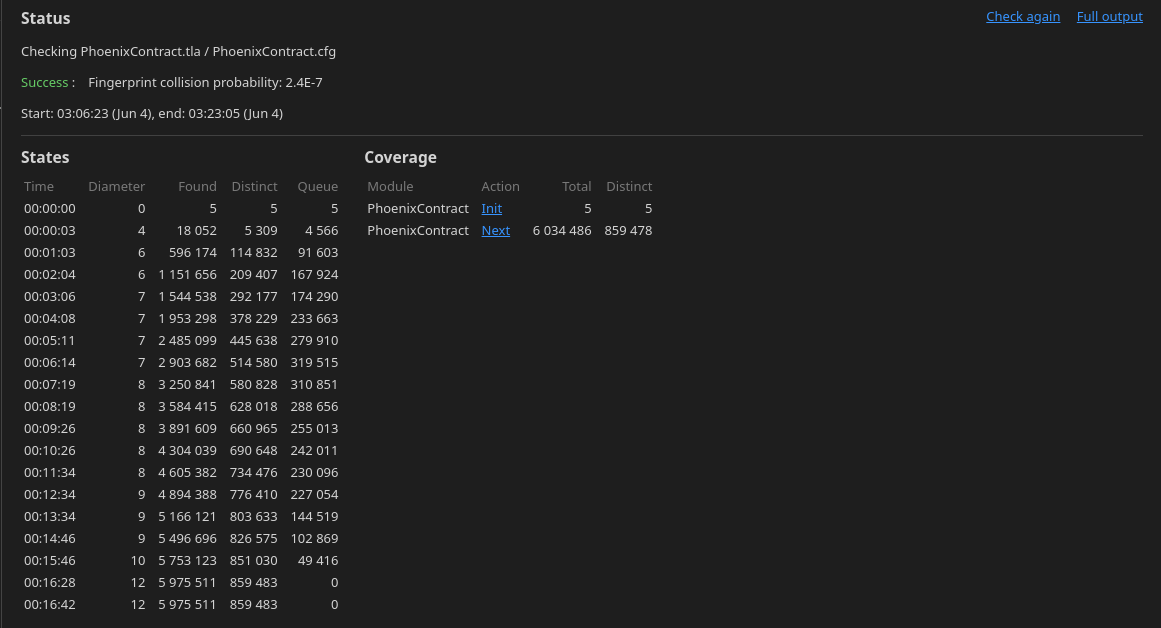
\includegraphics[width=12cm]{images/model_test.png}

\end{center}
\end{frame}

\begin{frame}
\frametitle{Результаты работы}

\begin{enumerate}
\item Построена и проверена модель контракта
\item Смоделированы атаки и потери ключей
\end{enumerate}

\vspace{5mm}\hrule

\begin{center}
\begin{tabularx}{0.9\textwidth}{ >{\raggedright\arraybackslash}l  >{\raggedleft\arraybackslash}X }
	 Владимир Рачкин \href{https://t.me/robozmey}{@robozmey} & \multirow{2}{4em}{
\includegraphics[width=2.8cm]{images/qr-code.png}} \\
Павел Балай \href{https://t.me/Koropok}{@Koropok} &  \\
Ссылка на Github проекта \href{https://github.com/robozmey/phoenix_proof}{phoenix\_proof}
\end{tabularx}
\end{center}



\end{frame}




\end{document}
